\documentclass[11pt,twoside]{article}\makeatletter

\IfFileExists{xcolor.sty}%
  {\RequirePackage{xcolor}}%
  {\RequirePackage{color}}
\usepackage{colortbl}
      
\usepackage{fontspec}
\usepackage{xunicode}
\catcode`⃥=\active \def⃥{\textbackslash}
\catcode`❴=\active \def❴{\{}
\catcode`❵=\active \def❵{\}}
\def\textJapanese{\fontspec{Kochi Mincho}}
\def\textChinese{\fontspec{HAN NOM A}\XeTeXlinebreaklocale "zh"\XeTeXlinebreakskip = 0pt plus 1pt }
\def\textKorean{\fontspec{Baekmuk Gulim} }
\setmonofont{DejaVu Sans Mono}

\DeclareTextSymbol{\textpi}{OML}{25}
\usepackage{relsize}
\def\textsubscript#1{%
  \@textsubscript{\selectfont#1}}
\def\@textsubscript#1{%
  {\m@th\ensuremath{_{\mbox{\fontsize\sf@size\z@#1}}}}}
\def\textquoted#1{‘#1’}
\def\textsmall#1{{\small #1}}
\def\textlarge#1{{\large #1}}
\def\textoverbar#1{\ensuremath{\overline{#1}}}
\def\textgothic#1{{\fontspec{Lucida Blackletter}#1}}
\def\textcal#1{{\fontspec{Lucida Calligraphy}#1}}
\RequirePackage{array}
\def\@testpach{\@chclass
 \ifnum \@lastchclass=6 \@ne \@chnum \@ne \else
  \ifnum \@lastchclass=7 5 \else
   \ifnum \@lastchclass=8 \tw@ \else
    \ifnum \@lastchclass=9 \thr@@
   \else \z@
   \ifnum \@lastchclass = 10 \else
   \edef\@nextchar{\expandafter\string\@nextchar}%
   \@chnum
   \if \@nextchar c\z@ \else
    \if \@nextchar l\@ne \else
     \if \@nextchar r\tw@ \else
   \z@ \@chclass
   \if\@nextchar |\@ne \else
    \if \@nextchar !6 \else
     \if \@nextchar @7 \else
      \if \@nextchar (8 \else
       \if \@nextchar )9 \else
  10
  \@chnum
  \if \@nextchar m\thr@@\else
   \if \@nextchar p4 \else
    \if \@nextchar b5 \else
   \z@ \@chclass \z@ \@preamerr \z@ \fi \fi \fi \fi
   \fi \fi  \fi  \fi  \fi  \fi  \fi \fi \fi \fi \fi \fi}

\gdef\arraybackslash{\let\\=\@arraycr}
\def\textxi{\ensuremath{\xi}}
\def\Panel#1#2#3#4{\multicolumn{#3}{){\columncolor{#2}}#4}{#1}}

\newcolumntype{L}[1]{){\raggedright\arraybackslash}p{#1}}
\newcolumntype{C}[1]{){\centering\arraybackslash}p{#1}}
\newcolumntype{R}[1]{){\raggedleft\arraybackslash}p{#1}}
\newcolumntype{P}[1]{){\arraybackslash}p{#1}}
\newcolumntype{B}[1]{){\arraybackslash}b{#1}}
\newcolumntype{M}[1]{){\arraybackslash}m{#1}}
\definecolor{label}{gray}{0.75}
\DeclareRobustCommand*{\xref}{\hyper@normalise\xref@}
\def\xref@#1#2{\hyper@linkurl{#2}{#1}}
\def\Div[#1]#2{\section*{#2}}
\begingroup
\catcode`\_=\active
\gdef_#1{\ensuremath{\sb{\mathrm{#1}}}}
\endgroup
\mathcode`\_=\string"8000
\catcode`\_=12\relax

\usepackage[a4paper,twoside,lmargin=1in,rmargin=1in,tmargin=1in,bmargin=1in]{geometry}
\usepackage{framed}

\definecolor{shadecolor}{gray}{0.95}
\usepackage{longtable}
\usepackage[normalem]{ulem}
\usepackage{fancyvrb}
\usepackage{fancyhdr}
\usepackage{marginnote}
\renewcommand*{\marginfont}{\itshape\footnotesize}
\setlength\marginparwidth{.75in}
\usepackage{graphicx}

\def\Gin@extensions{.pdf,.png,.jpg,.mps,.tif}

  \pagestyle{fancy} 

\usepackage[pdftitle={A Christmas Carol},
 pdfauthor={Dickens, Charles, 1812-1870}]{hyperref}
\hyperbaseurl{}

	 \paperwidth210mm
	 \paperheight297mm
              
\def\@pnumwidth{1.55em}
\def\@tocrmarg {2.55em}
\def\@dotsep{4.5}
\setcounter{tocdepth}{3}
\clubpenalty=8000
\emergencystretch 3em
\hbadness=4000
\hyphenpenalty=400
\pretolerance=750
\tolerance=2000
\vbadness=4000
\widowpenalty=10000

\renewcommand\section{\@startsection {section}{1}{\z@}%
     {-1.75ex \@plus -0.5ex \@minus -.2ex}%
     {0.5ex \@plus .2ex}%
     {\reset@font\Large\bfseries\sffamily}}
\renewcommand\subsection{\@startsection{subsection}{2}{\z@}%
     {-1.75ex\@plus -0.5ex \@minus- .2ex}%
     {0.5ex \@plus .2ex}%
     {\reset@font\Large\sffamily}}
\renewcommand\subsubsection{\@startsection{subsubsection}{3}{\z@}%
     {-1.5ex\@plus -0.35ex \@minus -.2ex}%
     {0.5ex \@plus .2ex}%
     {\reset@font\large\sffamily}}
\renewcommand\paragraph{\@startsection{paragraph}{4}{\z@}%
     {-1ex \@plus-0.35ex \@minus -0.2ex}%
     {0.5ex \@plus .2ex}%
     {\reset@font\normalsize\sffamily}}
\renewcommand\subparagraph{\@startsection{subparagraph}{5}{\parindent}%
     {1.5ex \@plus1ex \@minus .2ex}%
     {-1em}%
     {\reset@font\normalsize\bfseries}}


\def\l@section#1#2{\addpenalty{\@secpenalty} \addvspace{1.0em plus 1pt}
 \@tempdima 1.5em \begingroup
 \parindent \z@ \rightskip \@pnumwidth 
 \parfillskip -\@pnumwidth 
 \bfseries \leavevmode #1\hfil \hbox to\@pnumwidth{\hss #2}\par
 \endgroup}
\def\l@subsection{\@dottedtocline{2}{1.5em}{2.3em}}
\def\l@subsubsection{\@dottedtocline{3}{3.8em}{3.2em}}
\def\l@paragraph{\@dottedtocline{4}{7.0em}{4.1em}}
\def\l@subparagraph{\@dottedtocline{5}{10em}{5em}}
\@ifundefined{c@section}{\newcounter{section}}{}
\@ifundefined{c@chapter}{\newcounter{chapter}}{}
\newif\if@mainmatter 
\@mainmattertrue
\def\chaptername{Chapter}
\def\frontmatter{%
  \pagenumbering{roman}
  \def\thechapter{\@roman\c@chapter}
  \def\theHchapter{\alph{chapter}}
  \def\@chapapp{}%
}
\def\mainmatter{%
  \cleardoublepage
  \def\thechapter{\@arabic\c@chapter}
  \setcounter{chapter}{0}
  \setcounter{section}{0}
  \pagenumbering{arabic}
  \setcounter{secnumdepth}{6}
  \def\@chapapp{\chaptername}%
  \def\theHchapter{\arabic{chapter}}
}
\def\backmatter{%
  \cleardoublepage
  \setcounter{chapter}{0}
  \setcounter{section}{0}
  \setcounter{secnumdepth}{0}
  \def\@chapapp{\appendixname}%
  \def\thechapter{\@Alph\c@chapter}
  \def\theHchapter{\Alph{chapter}}
  \appendix
}
\newenvironment{bibitemlist}[1]{%
   \list{\@biblabel{\@arabic\c@enumiv}}%
       {\settowidth\labelwidth{\@biblabel{#1}}%
        \leftmargin\labelwidth
        \advance\leftmargin\labelsep
        \@openbib@code
        \usecounter{enumiv}%
        \let\p@enumiv\@empty
        \renewcommand\theenumiv{\@arabic\c@enumiv}%
	}%
  \sloppy
  \clubpenalty4000
  \@clubpenalty \clubpenalty
  \widowpenalty4000%
  \sfcode`\.\@m}%
  {\def\@noitemerr
    {\@latex@warning{Empty `bibitemlist' environment}}%
    \endlist}

\def\tableofcontents{\section*{\contentsname}\@starttoc{toc}}
\parskip0pt
\parindent1em
\def\Panel#1#2#3#4{\multicolumn{#3}{){\columncolor{#2}}#4}{#1}}
\newenvironment{reflist}{%
  \begin{raggedright}\begin{list}{}
  {%
   \setlength{\topsep}{0pt}%
   \setlength{\rightmargin}{0.25in}%
   \setlength{\itemsep}{0pt}%
   \setlength{\itemindent}{0pt}%
   \setlength{\parskip}{0pt}%
   \setlength{\parsep}{2pt}%
   \def\makelabel##1{\itshape ##1}}%
  }
  {\end{list}\end{raggedright}}
\newenvironment{sansreflist}{%
  \begin{raggedright}\begin{list}{}
  {%
   \setlength{\topsep}{0pt}%
   \setlength{\rightmargin}{0.25in}%
   \setlength{\itemindent}{0pt}%
   \setlength{\parskip}{0pt}%
   \setlength{\itemsep}{0pt}%
   \setlength{\parsep}{2pt}%
   \def\makelabel##1{\upshape\sffamily ##1}}%
  }
  {\end{list}\end{raggedright}}
\newenvironment{specHead}[2]%
 {\vspace{20pt}\hrule\vspace{10pt}%
  \hypertarget{#1}{}%
  \markright{#2}%

  \pdfbookmark[2]{#2}{#1}%
  \hspace{-0.75in}{\bfseries\fontsize{16pt}{18pt}\selectfont#2}%
  }{}
      
\@ifundefined{chapter}{%
    \def\DivI{\section}
    \def\DivII{\subsection}
    \def\DivIII{\subsubsection}
    \def\DivIV{\paragraph}
    \def\DivV{\subparagraph}
    \def\DivIStar[#1]#2{\section*{#2}}
    \def\DivIIStar[#1]#2{\subsection*{#2}}
    \def\DivIIIStar[#1]#2{\subsubsection*{#2}}
    \def\DivIVStar[#1]#2{\paragraph*{#2}}
    \def\DivVStar[#1]#2{\subparagraph*{#2}}
}{%
    \def\DivI{\chapter}
    \def\DivII{\section}
    \def\DivIII{\subsection}
    \def\DivIV{\subsubsection}
    \def\DivV{\paragraph}
    \def\DivIStar[#1]#2{\chapter*{#2}}
    \def\DivIIStar[#1]#2{\section*{#2}}
    \def\DivIIIStar[#1]#2{\subsection*{#2}}
    \def\DivIVStar[#1]#2{\subsubsection*{#2}}
    \def\DivVStar[#1]#2{\paragraph*{#2}}
}
\def\TheFullDate{}
\def\TheID{\makeatother }
\def\TheDate{}
\title{A Christmas Carol}
\author{Dickens, Charles, 1812-1870}\let\tabcellsep&
      \catcode`\&=12\relax \makeatletter 
\makeatletter
\thispagestyle{empty}
\markright{\@title}\markboth{\@title}{\@author}
\renewcommand\small{\@setfontsize\small{9pt}{11pt}\abovedisplayskip 8.5\p@ plus3\p@ minus4\p@
\belowdisplayskip \abovedisplayskip
\abovedisplayshortskip \z@ plus2\p@
\belowdisplayshortskip 4\p@ plus2\p@ minus2\p@
\def\@listi{\leftmargin\leftmargini
               \topsep 2\p@ plus1\p@ minus1\p@
               \parsep 2\p@ plus\p@ minus\p@
               \itemsep 1pt}
}
\makeatother
\fvset{frame=single,numberblanklines=false,xleftmargin=5mm,xrightmargin=5mm}
\fancyhf{} 
\setlength{\headheight}{14pt}
\fancyhead[LE]{\bfseries\leftmark} 
\fancyhead[RO]{\bfseries\rightmark} 
\fancyfoot[RO]{}
\fancyfoot[CO]{\thepage}
\fancyfoot[LO]{\TheID}
\fancyfoot[LE]{}
\fancyfoot[CE]{\thepage}
\fancyfoot[RE]{\TheID}
\hypersetup{linkbordercolor=0.75 0.75 0.75,urlbordercolor=0.75 0.75 0.75,bookmarksnumbered=true}
\fancypagestyle{plain}{\fancyhead{}\renewcommand{\headrulewidth}{0pt}}\makeatother 
\begin{document}

\catcode`\$=12\relax
\catcode`\^=12\relax
\catcode`\#=12\relax
\catcode`\%=12\relax
      \frontmatter 
\DivIStar[(half title note)]{(half title note)}\par
The Original Edition of A CHRISTMAS CAROL has been out of         print for many years, and this Edition is a reprint from the         stereotype plates of that Edition.
  \begin{titlepage}
  \title{A Christmas carol. in prose.  — being \textit{A Ghost Story of Christmas}}
  \maketitle
  by \author{Charles Dickens.}With illustrations by John Leech
  \end{titlepage}
  \cleardoublepage

\DivIStar[PREFACE]{PREFACE 	}\par
I have endeavoured in this Ghostly little book, to raise the 	Ghost of an Idea, which shall not put my readers out of humour 	with themselves, with each other, with the season, or with me. 	May it haunt their houses pleasantly, and no one wish to lay 	it. 
\begin{quote}
 Their faithful Friend and Servant, C.D. December, 1843.\end{quote}
\leftline{\textbf{Contents.}} \begin{description}

\item[Stave I]Marley's ghost \hyperlink{S1}{1}
\item[Stave II]The first of 	  the three spirits 
\item[Stave 	  III ]The second of the three spirits 
\item[Stave IV ]The last of 	  the spirits 
\item[Stave V]The end of it 
\end{description} \mainmatter 
\DivI[(Bits of) A CHRISTMAS CAROL, and other things]{(Bits of) A CHRISTMAS CAROL, and other things}
\DivI[Rendering tests]{Rendering tests}\par
‘Who-e debel 	  you?’ — he at last said —  	  ‘you no speak-e, 	  damme, I kill-e.’  And so saying, 	  the lighted tomahawk began flourishing 	  about me in the dark.\par
 	  ‘Who-e debel 	  you?’ — he at last said —  	  ‘you no speak-e, 	  damme, I kill-e.’  And so saying, 	  the lighted tomahawk began flourishing 	  about me in the dark.
\DivII[Quotations]{Quotations}\par
Consider quotations: 	‘This is a quote which is run on within the text and will  	have quote marks of some kind around it.’\par
Another quotation: 	\begin{quote}This is a block quote set off as such from the rest of the text\end{quote}\par
Here, by contrast is an ‘inline quotation’. Another strange thing  	about quotes is this: 	\begin{quote}You can put line breaks{\hskip1pt}\newline to determine where the line breaks{\hskip1pt}\newline Inside a block!\end{quote}\par
He used a French \textit{radiateur}.\par
Languages:  \textit{Deutsch};  \textit{Italiano};  \textit{Español};  \textit{Français};  \textit{Portugues};  \textit{Russian};  \textit{Svenska};  \textit{日本語};  \textit{中文}.
\DivII[Values of @rend on hi]{Values of @rend on \texttt{<hi>}} \par 
\begin{longtable}{P{0.1941044776119403\textwidth}P{0.6558955223880597\textwidth}}
\hline \rowcolor{label}Effect\tabcellsep Example\\\hline 
emph\tabcellsep This is \textit{emph} tag\\
hi\tabcellsep This is \textit{hi} tag\\
typewriter\tabcellsep This is \texttt{typewriter} effect\\
bold\tabcellsep This is \textbf{bold} effect\\
normalweight\tabcellsep This is {normalweight} effect\\
smallcaps\tabcellsep This is \textsc{smallcaps} effect\\
capsall\tabcellsep This is \uppercase{capsall} effect\\
strikethrough\tabcellsep This is \sout{strikethrough} effect\\
strikedoublethrough\tabcellsep This is {strikedoublethrough} effect\\
color(red)\tabcellsep This is \textcolor{red}{color(red)} effect\\
underline\tabcellsep This is \uline{underline} effect\\
underwavyline\tabcellsep This is \uwave{underwavyline} effect\\
underdoubleline\tabcellsep This is \uuline{underdoubleline} effect\\
subscript\tabcellsep This is \textsubscript{subscript} effect\\
superscript\tabcellsep This is \textsuperscript{superscript} effect\end{longtable} \par
 \par
{rend test 1}\footnote{Cairns 2003: 11. My work is Muellner 1996.}\par
{rend test 2}\footnote{Cairns 2003: 11. My work is Muellner 1996.}\par
A paragraph with a footnote containing a block-level 	object\footnote{We start with a quotation:
\leftline{This is the way the world ends}
\leftline{This is the way the world ends}
\leftline{This is the way the world ends}
\leftline{Not with a bang but a whimper.} which is from TS Eliot's \textit{Hollow men} } 
\DivII[del, gap, add, unclear etc]{del, gap, add, unclear etc}\par
. The \textsuperscript{interest} & — affor  	the amount \textbf{over}{\hskip1pt}\newline  so small the interest afforded 	compared with cash,  by the Annuity{\hskip1pt}\newline  note 	paper to those who \textbf{tutor} 	\textbf{think} it, or keep it, with a view {\hskip1pt}\newline  	to circulation, will, when compared with cash 	be it ever so small be {\hskip1pt}\newline  so much \uline{profit}: compared with a 	the preceding higher {\hskip1pt}\newline  rate of interest, the reduced 	rate afforded by the Annuity {\hskip1pt}\newline  note paper, to those who, 	\textbf{tutor} if they \textbf{tutor} it, 	{\hskip1pt}\newline  will, have to depend upon to the extent of their {\hskip1pt}\newline  	respective capitals so invested, have nothing else {\hskip1pt}\newline  to depend upon for 	their respective incomes, will,  	by the {\hskip1pt}\newline  amount of the difference, \textbf{foremost} 	itself as so {\hskip1pt}\newline  much less.
\DivII[And now for something dramatic...]{And now for something dramatic...} \begin{description} \item[Roderigo] 

Where shall we meet i' the morning?\end{description}
 \begin{description} \item[Iago] 

At my lodging.\end{description}
 \begin{description} \item[Roderigo] 

I'll be with thee betimes.\end{description}
 \begin{description} \item[Iago] 

Go to; farewell. Do you hear, Roderigo?\end{description}
 \begin{description} \item[Roderigo] 

What say you?\end{description}
 \begin{description} \item[Iago] 

No more of drowning, do you hear?\end{description}
 \begin{description} \item[Roderigo] 

I am changed: I'll go sell all my land.\end{description}

\DivII[Footnotes]{Footnotes}
\DivIII[1 Zur Entstehung der Philosophischen UntersuchungenZu Textauszeichnungen und Siglen siehe die Legende.]{1 Zur Entstehung der {Philosophischen  	Untersuchungen}\footnote{Zu Textauszeichnungen und  	Siglen siehe die Legende.}}\par
Iriure dolor in hendrerit in vulputate velit esse molestie       consequat, vel illum dolore eu feugiat nulla facilisis at vero eros et       accumsan et iusto odio dignissim qui blandit praesent luptatum zzril       delenit augue duis dolore te feugait nulla facilisi. Lorem ipsum dolor       sit amet, consectetuer adipiscing elit, sed diam nonummy nibh euismod 	\footnote{Zu  	Textauszeichnungen und Siglen siehe die Legende.}       Iriure dolor in hendrerit in vulputate velit esse molestie       consequat, vel illum dolore eu feugiat nulla facilisis at vero eros et       accumsan et iusto odio dignissim qui blandit praesent luptatum zzril       delenit augue duis dolore te feugait nulla facilisi. Lorem ipsum dolor       sit amet, consectetuer adipiscing elit, sed diam nonummy nibh euismod
\DivII[emph and links]{emph and links}\par
The \texttt{<emph>} element is used for linguistic           emph\textit{asis}.  ‘highlighting’           (\texttt{<soCalled>}) nor with \emph{shouting}           (\texttt{<mentioned>}), \emph{transmogrification}, (a           technical \texttt{<term>}), for which the \texttt{<gloss>} tag           might be used to supply  \textit{a technical           definition}).\par
Now for some links! We will start by cross-referring to a later section.\par
Here is a simple             \texttt{<ptr>}             to it:             \textit{\hyperref[P1]{1.8. Lists}}. Here is a simple             \texttt{<ref>}, a             \hyperlink{P1}{reference to it}.\par
An             \xref{http://www.bbc.co.uk}{external link}             as ref and as ptr:             \url{http://www.bbc.co.uk}.
\DivII[Tables]{Tables}\par
Tables may have cells that span multiple columns and rows. \par 
\begin{longtable}{P{0.5995698924731182\textwidth}P{0.18645161290322582\textwidth}P{0.06397849462365592\textwidth}}
 \hline\endfoot\hline\endlastfoot \endfirsthead \multicolumn{3}{c}{Pictures from Fagaras mountains(cont.)}\\\hline \endhead \caption{Pictures from Fagaras mountains}\\ \hline \rowcolor{label}Image\tabcellsep Description\tabcellsep Camera direction\\\hline 
SVG, JPEG, GIF or PNG format\\
\Panel{               \textit{All pictures were taken on Jun 27, 2007               }             }{label}{2}{l}\\
               \noindent
\includegraphics[]{nature1.jpg}             \tabcellsep Mountain flowers.             \tabcellsep north\\
               \noindent
\includegraphics[]{nature2.jpg}             \tabcellsep Sunset over a secondary ridge.\tabcellsep north-east\\
               \noindent
\includegraphics[]{nature3.jpg}             \tabcellsep Glacier lake at 2100m altitude.\tabcellsep east\end{longtable} \par
  \par 
\begin{longtable}{P{0.3334140435835351\textwidth}P{0.15641646489104116\textwidth}P{0.18523002421307505\textwidth}P{0.1708232445520581\textwidth}P{0.004116222760290557\textwidth}}
 \hline\endfoot\hline\endlastfoot \endfirsthead \multicolumn{3}{c}{
            TEI Span Sample
          (cont.)}\\\hline \endhead \caption{
            TEI Span Sample
          }\\ \hline \rowcolor{label}\multicolumn{2}{){\columncolor{label}}l}{Spans                             \textbf{Horizontally}                         }\tabcellsep Header 3\tabcellsep \multicolumn{2}{){\columncolor{label}}l}{Spans                             \textbf{Horizontally}                         }\\\hline 
Spans                             \textbf{Vertically}                         \tabcellsep a\tabcellsep b\tabcellsep c\tabcellsep d\\
e\tabcellsep \multicolumn{2}{l}{Spans                             \textbf{both}                         }\tabcellsep f\\
g\tabcellsep g\\
i\tabcellsep j\tabcellsep \multicolumn{2}{l}{Spans                             \textbf{Horizontally}                         }\\
k\tabcellsep l\tabcellsep m\tabcellsep n\tabcellsep o\end{longtable} \par
 
\DivII[Lists]{Lists}\label{P1}\par
Various sorts of list are legal within paragraphs...           \begin{enumerate}

\item Dogs
\item Zebras
\item Birds
\item Cats
\end{enumerate}         \begin{description}

\item[100]first item           
\item[200]second item           
\item[300]third item           
\end{description} \par
The preceding lists was between paragraphs.\par
           \leftline{\textbf{This untyped list has a heading and a nested glosslist             }} \begin{itemize}

\item first item             
\item                \begin{description}

\item[25]first item                 
\item[35]second item                 
\item[45]third item                 
\end{description}              
\item third item             
\end{itemize}          
\DivI[MARLEY'S GHOST]{MARLEY'S GHOST}\label{S1}\par
Marley was dead: to begin with.  There is no doubt whatever about that.  The register of his burial was signed by the clergyman, the clerk, the undertaker, and the chief mourner.  Scrooge signed it.  And Scrooge's name was good upon 'Change, for anything he chose to put his hand to.  Old Marley was as dead as a door-nail.  \par
Mind!  I don't mean to say that I know, of my own knowledge, what there is particularly dead about a door-nail. I might have been inclined, myself, to regard a coffin-nail as the deadest piece of ironmongery in the trade.  But the wisdom of our ancestors is in the simile; and my unhallowed  hands shall not disturb it, or the Country's done for.  You will therefore permit me to repeat, emphatically, that Marley was as dead as a door-nail.  \par
Scrooge knew he was dead?  Of course he did.  How could it be otherwise?  Scrooge and he were partners for I don't know how many years.  Scrooge was his sole executor, his sole administrator, his sole assign, his sole residuary legatee, his sole friend, and sole mourner.  And even Scrooge was not so dreadfully cut up by the sad event, but that he was an excellent man of business on the very day of the funeral, and solemnised it with an undoubted bargain.  \par
The mention of Marley's funeral brings me back to the point I started from.  There is no doubt that Marley was dead.  This must be distinctly understood, or nothing wonderful can come of the story I am going to relate.  If we were not perfectly convinced that Hamlet's Father died before the play began, there would be nothing more remarkable in his taking a stroll at night, in an easterly wind, upon his own ramparts, than there   would be in any other middle-aged gentleman rashly  turning out after dark in a breezy spot — say Saint  Paul's Churchyard for instance — literally to astonish his son's weak mind.  \par
Scrooge never painted out Old Marley's name.  There it stood, years afterwards, above the ware-house door: Scrooge and Marley.  The firm was known as Scrooge and Marley. Sometimes people new to the business called Scrooge Scrooge, and sometimes Marley, but he answered to both names.  It was all the same to him.  \par
Oh!  But he was a tight-fisted hand at the grindstone, Scrooge!  a squeezing, wrenching, grasping, scraping, clutching, covetous old sinner!  Hard and sharp as flint, from which no steel had ever struck out generous fire; secret, and self-contained, and solitary as an oyster.  The cold within him froze his old features, nipped his pointed nose, shrivelled his cheek, stiffened his gait; made his eyes red, his thin lips blue; and spoke out shrewdly in his grating voice.  A frosty rime was on his head, and on his eyebrows, and his wiry chin. He   carried his own low temperature always about with him; he iced his office in the dog-days; and didn't thaw it one degree at Christmas.  \par
External heat and cold had little influence on Scrooge. No warmth could warm, no wintry weather chill him.  No wind that blew was bitterer than he, no falling snow was more intent upon its purpose, no pelting rain less open to entreaty. Foul weather didn't know where to have him.  The heaviest rain, and snow, and hail, and sleet, could boast of the advantage over him in only one respect.  They often ‘came down’ handsomely, and Scrooge never did.  \par
Nobody ever stopped him in the street to say, with gladsome looks, ‘My dear Scrooge, how are you.  When will you come to see me.’  No beggars implored him to bestow a trifle, no children asked him what it was o'clock, no man or woman ever once in all his life inquired the way to such and such a place, of Scrooge.  Even the blindmen's dogs appeared to know him; and when they saw him coming on, would tug their owners into doorways  and up courts; and then would wag their tails as though they said, ‘No eye at all is better than an evil eye, dark master! ’  \par
But what did Scrooge care!  It was the very thing he liked.  To edge his way along the crowded paths of life, warning all human sympathy to keep its distance, was what the knowing ones call ‘nuts’ to Scrooge.  \par
Once upon a time — of all the good days in the year, on Christmas Eve — old Scrooge sat busy in his counting-house. It was cold, bleak, biting weather: foggy withal: and he could hear the people in the court outside, go wheezing up and down, beating their hands upon their breasts, and stamping their feet upon the pavement stones to warm them. The city clocks had only just gone three, but it was quite dark already: it had not been light all day: and candles were flaring in the windows of the neighbouring offices, like ruddy smears upon the palpable brown air.  The fog came pouring in at every chink and keyhole, and was so dense without, that although the court was of the   narrowest, the houses opposite were mere phantoms.  To see the dingy cloud come drooping down, obscuring everything, one might have thought that Nature lived hard by, and was brewing on a large scale.  \par
The door of Scrooge's counting-house was open that he might keep his eye upon his clerk, who in a dismal little cell beyond, a sort of tank, was copying letters.  Scrooge had a very small fire, but the clerk's fire was so very much smaller that it looked like one coal.  But he couldn't replenish it, for Scrooge kept the coal-box in his own room; and so surely as the clerk came in with the shovel, the master predicted that it would be necessary for them to part.  Wherefore the clerk put on his white comforter, and tried to warm himself at the candle; in which effort, not being a man of a strong imagination, he failed.  \par
‘A merry Christmas, uncle!  God save you!’ cried a cheerful voice.  It was the voice of Scrooge's nephew, who came upon him so quickly that this was the first intimation he had of his approach.   \par
‘Bah!’ said Scrooge, ‘Humbug!’  \par
He had so heated himself with rapid walking in the fog and frost, this nephew of Scrooge's, that he was all in a glow; his face was ruddy and handsome; his eyes sparkled, and his breath smoked again.  \par
‘Christmas a humbug, uncle!’ said Scrooge's nephew.  ‘You don't mean that, I am sure.’  \par
‘I do,’ said Scrooge.  ‘Merry Christmas!  What right have you to be merry?  what reason have you to be merry? You're poor enough.’  \par
‘Come, then,’ returned the nephew gaily.  ‘What right have you to be dismal?  what reason have you to be morose? You're rich enough.’  \par
Scrooge having no better answer ready on the spur of the moment, said, ‘Bah!’ again; and followed it up with  ‘Humbug.’  \par
‘Don't be cross, uncle,’ said the nephew.  \par
‘What else can I be,’ returned the uncle, ‘when I live in such a world of fools as this  Merry Christmas!  Out upon merry Christmas.  What's Christmas time to you but a time for  paying bills without money; a time for finding yourself a year older, but not an hour richer; a time for balancing your books and having every item in 'em through a round dozen of months presented dead against you?  If I could work my will,’ said Scrooge indignantly, ‘every idiot who goes about with ‘Merry Christmas’ on his lips, should be boiled with his own pudding, and buried with a stake of holly through his heart.  He should!’  \par
‘Uncle!’ pleaded the nephew.  \par
‘Nephew!’ returned the uncle, sternly, ‘keep Christmas in your own way, and let me keep it in mine.’  \par
‘Keep it!’ repeated Scrooge's nephew.  ‘But you don't keep it.’  \par
‘Let me leave it alone, then,’ said Scrooge.  ‘Much good may it do you!  Much good it has ever done you!’  \par
‘There are many things from which I might have derived good, by which I have not profited, I dare say,’ returned the nephew:  ‘Christmas among the rest.  But I am sure I have always thought of Christmas time, when it has come round  — apart from the veneration due to its sacred name and origin, if anything belonging to it can be apart from that — as a good time: a kind, forgiving, charitable, pleasant time: the only time I know of, in the long calendar of the year, when men and women seem by one consent to open their shut-up hearts freely, and to think of people below them as if they really were fellow-passengers to the grave, and not another race of creatures bound on other journeys.  And therefore, uncle, though it has never put a scrap of gold or silver in my pocket, I believe that it \textit{has} done me good, and \textit{will} do me good; and I say, God bless it!’  \par
The clerk in the tank involuntarily applauded.  Becoming immediately sensible of the impropriety, he poked the fire, and extinguished the last frail spark for ever.  \par
‘Let me hear another sound from \textit{you},’ said Scrooge,  ‘ and you'll keep your Christmas by losing your situation. You're quite a powerful speaker, sir,’ he added, turning to his nephew.  ‘I wonder you don't go into Parliament.’  \par
           ‘Don't be angry, uncle.  Come!  Dine with us to-morrow.’         \par
Scrooge said that he would see him — yes, indeed he did. He went the whole length of the expression, and said that he would see him in that extremity first.  \par
‘But why?’ cried Scrooge's nephew.  ‘Why?’  \par
‘Why did you get married?’ said Scrooge.  \par
           ‘Because I fell in love.’         \par
‘Because you fell in love!’ growled Scrooge, as if that were the only one thing in the world more ridiculous than a merry Christmas.  ‘Good afternoon!’  \par
           ‘Nay, uncle, but you never came to see me before that happened.  Why give it as a reason for not coming now?’         \par
‘Good afternoon,’ said Scrooge.  \par
           ‘I want nothing from you; I ask nothing of you; why cannot we be friends?’         \par
‘Good afternoon,’ said Scrooge.  \par
           ‘I am sorry, with all my heart, to find you so resolute. We have never had any quarrel, to which I have been a party.  But I have made the trial in homage to Christmas, and I'll keep my Christmas humour to the last.  So A Merry Christmas, uncle!’         \par
‘Good afternoon!’ said Scrooge.  \par
           ‘And A Happy New Year!’         \par
‘Good afternoon!’ said Scrooge.  \par
His nephew left the room without an angry word, notwithstanding. He stopped at the outer door to bestow the greeting of the season on the clerk, who, cold as he was, was warmer than Scrooge; for he returned them cordially.  \par
‘There's another fellow,’ muttered Scrooge; who overheard him: ‘my clerk, with fifteen shillings a week, and a wife and family, talking about a merry Christmas.  I'll retire to Bedlam.’  \par
This lunatic, in letting Scrooge's nephew out, had let two other people in.  They were portly gentlemen, pleasant to behold, and now stood, with their hats off, in Scrooge's office. They had books and papers in their hands, and bowed to him.  \par
‘Scrooge and Marley's, I believe,’ said one of the  gentlemen, referring to his list.  ‘Have I the pleasure of addressing Mr Scrooge, or Mr Marley?’  \par
‘Mr Marley has been dead these seven years,’ Scrooge replied. ‘He died seven years ago, this very night.’  \par
‘We have no doubt his liberality is well represented by his surviving partner,’ said the gentleman, presenting his credentials.  \par
It certainly was; for they had been two kindred spirits. At the ominous word ‘liberality’, Scrooge frowned, and shook his head, and handed the credentials back.  \par
‘At this festive season of the year, Mr Scrooge,’ said the gentleman, taking up a pen, ‘it is more than usually desirable that we should make some slight provision for the Poor and destitute, who suffer greatly at the present time.  Many thousands are in want of common necessaries; hundreds of thousands are in want of common comforts, sir.’  \par
‘Are there no prisons?’ asked Scrooge.  \par
‘Plenty of prisons,’ said the gentleman, laying down the pen again.   \par
‘And the Union workhouses?’ demanded Scrooge.  ‘Are they still in operation?’  \par
‘They are.  Still,’ returned the gentleman, ‘ I wish I could say they were not.’  \par
‘The Treadmill and the Poor Law are in full vigour, then?’ said Scrooge.  \par
           ‘Both very busy, sir.’         \par
‘Oh!  I was afraid, from what you said at first, that something had occurred to stop them in their useful course,’ said Scrooge.  ‘I'm very glad to hear it.’  \par
‘Under the impression that they scarcely furnish Christian cheer of mind or body to the multitude,’ returned the gentleman, ‘a few of us are endeavouring to raise a fund to buy the Poor some meat and drink, and means of warmth. We choose this time, because it is a time, of all others, when Want is keenly felt, and Abundance rejoices.  What shall I put you down for?’  \par
‘Nothing!’ Scrooge replied.  \par
           ‘You wish to be anonymous?’         \par
‘I wish to be left alone,’ said Scrooge.  ‘Since  you ask me what I wish, gentlemen, that is my answer.  I don't make merry myself at Christmas and I can't afford to make idle people merry.  I help to support the establishments I have mentioned: they cost enough: and those who are badly off must go there.’  \par
           ‘Many can't go there; and many would rather die.’         \par
‘If they would rather die,’ said Scrooge, ‘they had better do it, and decrease the surplus population.  Besides — excuse me — I don't know that.’  \par
‘But you might know it,’ observed the gentleman.  \par
‘It's not my business,’ Scrooge returned.  ‘It's enough for a man to understand his own business, and not to interfere with other people's.  Mine occupies me constantly. Good afternoon, gentlemen!’  \par
Seeing clearly that it would be useless to pursue their point, the gentlemen withdrew.  Scrooge resumed his labours with an improved opinion of himself, and in a more facetious temper than was usual with him.   \par
Meanwhile the fog and darkness thickened so, that people ran about with flaring links, proffering their services to go before horses in carriages, and conduct them on their way. The ancient tower of a church, whose gruff old bell was always peeping slily down at Scrooge out of a gothic window in the wall, became invisible, and struck the hours and quarters in the clouds, with tremulous vibrations afterwards as if its teeth were chattering in its frozen head up there. The cold became intense.  In the main street, at the corner of the court, some labourers were repairing the gas-pipes, and had lighted a great fire in a brazier, round which a party of ragged men and boys were gathered: warming their hands and winking their eyes before the blaze in rapture. The water-plug being left in solitude, its overflowings sullenly congealed, and turned to misanthropic ice.  The brightness of the shops where holly sprigs and berries crackled in the lamp-heat of the windows, made pale faces ruddy as they passed.  Poulterers' and grocers' trades became a splendid joke: a glorious pageant, with which it was next to impossible to believe that such dull principles as bargain and sale had anything to do.  The Lord Mayor, in the stronghold of the might Mansion House, gave orders to his fifty cooks and butlers to keep Christmas as a Lord Mayor's household should; and even the little tailor, whom he had fined five shillings on the previous Monday for being drunk and bloodthirsty in the streets, stirred up tomorrow's pudding in his garret, while his lean wife and the baby sallied out to buy the beef.  \par
Foggier yet, and colder!  Piercing, searching, biting cold. If the good Saint Dunstan had but nipped the Evil Spirit's nose with a touch of such weather as that,  {\small\itshape [Note: test of a note]}  instead of using his familiar weapons, then indeed he would have roared to lusty purpose.  The owner of one scant young nose, gnawed and mumbled by the hungry cold as bones are gnawed by dogs, stooped down at Scrooge's keyhole to regale him with a Christmas carol: but at the first sound of  
\begin{quote}
\leftline{God bless you, merry gentleman! }
\leftline{May nothing you dismay! }\end{quote}
 Scrooge seized the ruler with such energy of action that the singer fled in terror, leaving the keyhole to the fog and even more congenial frost.  \par
At length the hour of shutting up the counting-house arrived.  With an ill-will Scrooge dismounted from his stool, and tacitly admitted the fact to the expectant clerk in the Tank, who instantly snuffed his candle out, and put on his hat.  \par
‘You'll want all day tomorrow, I suppose?’ said Scrooge.  \par
           ‘If quite convenient, Sir.’         \par
‘It's not convenient,’ said Scrooge, ‘and it's not fair. If I was to stop half-a-crown for it, you'd think yourself ill-used, I 'll be bound?’  \par
The clerk smiled faintly.  \par
‘And yet,’ said Scrooge, ‘you don't think \textit{me} ill-used, when I pay a day's wages for no work.’  \par
The clerk observed that it was only once a year.  \par
‘A poor excuse for picking a man's pocket every twenty-fifth of December!’ said Scrooge, buttoning his great-coat to the chin.  ‘But I suppose you must have the whole day. Be here all the earlier next morning!’   \par
The clerk promised that he would; and Scrooge walked out with a growl.  The office was closed in a twinkling, and the clerk, with the long ends of his white comforter dangling below his waist (for he boasted no great-coat), went down a slide on Cornhill, at the end of a lane of boys, twenty times, in honour of its being Christmas Eve, and then ran home to Camden Town as hard as he could pelt, to play at blindman's buff.  \par
Scrooge took his melancholy dinner in his usual melancholy tavern; and having read all the newspapers, and beguiled the rest of the evening with his banker's-book, went home to bed.  He lived in chambers which had once belonged to his deceased partner.  They were a gloomy suite of rooms, in a lowering pile of building up a yard, where it had so little business to be, that one could scarcely help fancying it must have run there when it was a young house, playing at hide-and-seek with other houses, and have forgotten the way out again. It was old enough now, and dreary enough, for nobody lived in it but Scrooge, the other rooms being all let out as offices. The yard was so dark that even Scrooge, who knew its every stone, was fain to grope with his hands.  The fog and frost so hung about the black old gateway of the house, that it seemed as if the Genius of the Weather sat in mournful meditation on the threshold.  \par
Now, it is a fact, that there was nothing at all particular about the knocker on the door, except that it was very large. It is also a fact, that Scrooge had seen it, night and morning, during his whole residence in that place; also that Scrooge had as little of what is called fancy about him as any man in the City of London, even including — which is a bold word — the corporation, aldermen, and livery.  Let it also be borne in mind that Scrooge had not bestowed one thought on Marley, since his last mention of his seven-year's dead partner that afternoon.  And then let any man explain to me, if he can, how it happened that Scrooge, having his key in the lock of the door, saw in the knocker, without its undergoing any intermediate process of change:  not a knocker, but Marley's face.   \par
Marley's face.  It was not in impenetrable shadow as the other objects in the yard were, but had a dismal light about it, like a bad lobster in a dark cellar.  It was not angry or ferocious, but looked at Scrooge as Marley used to look: with ghostly spectacles turned up upon its ghostly forehead. The hair was curiously stirred, as if by breath or hot-air; and, though the eyes were wide open, they were perfectly motionless.  That, and its livid colour, made it horrible; but its horror seemed to be in spite of the face and beyond its control, rather than a part of its own expression.  \par
As Scrooge looked fixedly at this phenomenon, it was a knocker again.  \par
To say that he was not startled, or that his blood was not conscious of a terrible sensation to which it had been a stranger from infancy, would be untrue.  But he put his hand upon the key he had relinquished, turned it sturdily, walked in, and lighted his candle.  \par
He \textit{did} pause, with a moment's irresolution, before he shut the door; and he \textit{did} look cautiously behind it first, as if he half expected to be terrified with the sight of Marley's pigtail sticking out into the hall.  But there was nothing on the back of the door, except the screws and nuts that held the knocker on, so he said ‘Pooh, pooh!’ and closed it with a bang.  \par
The sound resounded through the house like thunder. Every room above, and every cask in the wine-merchant's cellars below, appeared to have a separate peal of echoes of its own.  Scrooge was not a man to be frightened by echoes. He fastened the door, and walked across the hall, and up the stairs, slowly too: trimming his candle as he went.  \par
You may talk vaguely about driving a coach-and-six up a good old flight of stairs, or through a bad young Act of Parliament; but I mean to say you might have got a hearse up that staircase, and taken it broadwise, with the splinter-bar towards the wall and the door towards the balustrades: and done it easy.  There was plenty of width for that, and room to spare; which is perhaps the reason why Scrooge thought he saw a locomotive hearse going on before him in the gloom. Half-a-dozen gas-lamps out of the street wouldn't have lighted the entry too well, so you may suppose that it was pretty dark with Scrooge's dip.  \par
Up Scrooge went, not caring a button for that: darkness is cheap, and Scrooge liked it.  But before he shut his heavy door, he walked through his rooms to see that all was right. He had just enough recollection of the face to desire to do that.  \par
Sitting-room, bed-room, lumber-room.  All as they should be.  Nobody under the table, nobody under the sofa; a small fire in the grate; spoon and basin ready; and the little saucepan of gruel (Scrooge has a cold in his head) upon the hob. Nobody under the bed; nobody in the closet; nobody in his dressing-gown, which was hanging up in a suspicious attitude against the wall.  Lumber-room as usual.  Old fire-guard, old shoes, two fish-baskets, washing-stand on three legs, and a poker.  \par
Quite satisfied, he closed his door, and locked himself in; double-locked himself in, which was not his custom.  Thus secured against surprise, he took off his cravat; put on his dressing-gown and slippers, and his night-cap; and sat down before the fire to take his gruel.  \par
It was a very low fire indeed; nothing on such a bitter night.  He was obliged to sit close to it, and brood over it, before he could extract the least sensation of warmth from such a handful of fuel.  The fireplace was an old one, built by some Dutch merchant long ago, and paved all round with quaint Dutch tiles, designed to illustrate the Scriptures. There were Cains and Abels, Pharaoh's daughters, Queens of Sheba, Angelic messengers descending through the air on clouds like feather-beds, Abrahams, Belshazzars, Apostles putting off to sea in butter-boats, hundreds of figures to attract his thoughts; and yet that face of Marley, seven years dead, came like the ancient Prophet's rod, and swallowed up the whole.  If each smooth tile had been a blank at first, with power to shape some picture on its surface from the disjointed fragments of his thoughts, there would have been a copy of old Marley's head on every one.   \par
‘Humbug!’ said Scrooge; and walked across the room.  \par
After several turns, he sat down again.  As he threw his head back in the chair, his glance happened to rest upon a bell, a disused bell, that hung in the room, and communicated for some purpose now forgotten with a chamber in the highest story of the building.  It was with great astonishment, and with a strange, inexplicable dread, that as he looked, he saw this bell begin to swing.  It swung so softly in the outset that it scarcely made a sound; but soon it rang out loudly, and so did every bell in the house.  \par
This might have lasted half a minute, or a minute, but it seemed an hour.  The bells ceased as they had begun, together.  They were succeeded by a clanking noise, deep down below; as if some person were dragging a heavy chain over the casks in the wine-merchant's cellar.  Scrooge then remembered to have heard that ghosts in haunted houses were described as dragging chains.  \par
The cellar-door flew open with a booming sound, and then he heard the noise much louder, on the floors below; then coming up the stairs; then coming straight towards his door.  \par
‘It's humbug still!’ said Scrooge.  ‘I won't believe it.’  \par
His colour changed though, when, without a pause, it came on through the heavy door, and passed into the room before his eyes.  Upon its coming in, the dying flame leaped up, as though it cried, ‘I know him! Marley's Ghost!’ and fell again.  \par
The same face: the very same.  Marley in his pigtail, usual waistcoat, tights, and boots; the tassels on the latter bristling, like his pigtail, and his coat-skirts, and the hair upon his head.  The chain he drew was clasped about his middle.  It was long, and wound about him like a tail; and it was made (for Scrooge observed it closely) of cash-boxes, keys, padlocks, ledgers, deeds, and heavy purses wrought in steel.  His body was transparent; so that Scrooge, observing him, and looking through his waistcoat, could see the two buttons on his coat behind.   \par
Scrooge had often heard it said that Marley had no bowels, but he had never believed it until now.  \par
No, nor did he believe it even now.  Though he looked the phantom through and through, and saw it standing before him; though he felt the chilling influence of its death-cold eyes; and marked the very texture of the folded kerchief bound about its head and chin, which wrapper he had not observed before; he was still incredulous, and fought against his senses.  \par
‘How now!’ said Scrooge, caustic and cold as ever.  ‘What do you want with me?’  \par
‘Much!’ — Marley's voice, no doubt about it.  \par
           ‘Who are you?’         \par
           ‘Ask me who I \textit{was}.’         \par
‘Who \textit{were} you then.’ said Scrooge, raising his voice.  ‘You're particular, for a shade.’ He was going to say ‘\textit{to} a shade,’ but substituted this, as more appropriate.  \par
           ‘In life I was your partner, Jacob Marley.’         \par
‘Can you — can you sit down?’ asked Scrooge, looking doubtfully at him.   \par
           ‘I can.’         \par
           ‘Do it, then.’         \par
Scrooge asked the question, because he didn't know whether a ghost so transparent might find himself in a condition to take a chair; and felt that in the event of its being impossible, it might involve the necessity of an embarrassing explanation. But the ghost sat down on the opposite side of the fireplace, as if he were quite used to it.  \par
‘You don't believe in me,’ observed the Ghost.  \par
‘I don't,’ said Scrooge.  \par
           ‘What evidence would you have of my reality beyond that of your senses?’         \par
‘I don't know,’ said Scrooge.  \par
           ‘Why do you doubt your senses?’         \par
‘Because,’ said Scrooge, ‘a little thing affects them.  A slight disorder of the stomach makes them cheats.  You may be an undigested bit of beef, a blot of mustard, a crumb of cheese, a fragment of an underdone potato.  There's more of gravy than of grave about you, whatever you are!’  \par
Scrooge was not much in the habit of cracking jokes, nor did he feel, in his heart, by any means waggish then.  The truth is, that he tried to be smart, as a means of distracting his own attention, and keeping down his terror; for the spectre's voice disturbed the very marrow in his bones.  \par
To sit, staring at those fixed, glazed eyes, in silence for a moment, would play, Scrooge felt, the very deuce with him. There was something very awful, too, in the spectre's being provided with an infernal atmosphere of its own.  Scrooge could not feel it himself, but this was clearly the case; for though the Ghost sat perfectly motionless, its hair, and skirts, and tassels, were still agitated as by the hot vapour from an oven.  \par
‘You see this toothpick?’ said Scrooge, returning quickly to the charge, for the reason just assigned; and wishing, though it were only for a second, to divert the vision's stony gaze from himself.  \par
‘I do,’ replied the Ghost.  \par
‘You are not looking at it,’ said Scrooge.  \par
‘But I see it,’ said the Ghost, ‘notwithstanding.’  \par
‘Well!’ returned Scrooge, ‘I have but to swallow this, and be for the rest of my days persecuted by a legion of goblins, all of my own creation.  Humbug, I tell you; humbug!’  \par
At this the spirit raised a frightful cry, and shook its chain with such a dismal and appalling noise, that Scrooge held on tight to his chair, to save himself from falling in a swoon. But how much greater was his horror, when the phantom taking off the bandage round its head, as if it were too warm to wear in-doors, its lower jaw dropped down upon its breast!  \par
Scrooge fell upon his knees, and clasped his hands before his face.  \par
‘Mercy!’ he said.  ‘Dreadful apparition, why do you trouble me?’  \par
‘Man of the worldly mind!’ replied the Ghost, ‘do you believe in me or not?’  \par
‘I do,’ said Scrooge.  ‘I must.  But why do spirits walk the earth, and why do they come to me?’  \par
‘It is required of every man,’ the Ghost returned, ‘that the spirit within him should walk abroad among his fellow-men, and travel far and wide; and if that spirit goes not forth in life, it is condemned to do so after death.  It is doomed to wander through the world — oh, woe is me! — and witness what it cannot share, but might have shared on earth, and turned to happiness!’  \par
Again the spectre raised a cry, and shook its chain, and wrung its shadowy hands.  \par
‘You are fettered,’ said Scrooge, trembling.  ‘Tell me why?’  \par
‘I wear the chain I forged in life,’ replied the Ghost.  ‘I made it link by link, and yard by yard; I girded it on of my own free will, and of my own free will I wore it.  Is its pattern strange to \textit{you}?’  \par
Scrooge trembled more and more.  \par
‘Or would you know,’ pursued the Ghost, ‘the weight and length of the strong coil you bear yourself?  It was full as heavy and as long as this, seven Christmas Eves ago.  You have laboured on it, since.  It is a ponderous chain!’  \par
Scrooge glanced about him on the floor, in the expectation of finding himself surrounded by some fifty or sixty fathoms of iron cable: but he could see nothing.  \par
‘Jacob,’ he said, imploringly.  ‘Old Jacob Marley, tell me more.  Speak comfort to me, Jacob.’  \par
‘I have none to give,’ the Ghost replied.  ‘It comes from other regions, Ebenezer Scrooge, and is conveyed by other ministers, to other kinds of men.  Nor can I tell you what I would.  A very little more, is all permitted to me.  I cannot rest, I cannot stay, I cannot linger anywhere.  My spirit never walked beyond our counting-house — mark me! — in life my spirit never roved beyond the narrow limits of our money-changing hole; and weary journeys lie before me!’  \par
It was a habit with Scrooge, whenever he became thoughtful, to put his hands in his breeches pockets.  Pondering on what the Ghost had said, he did so now, but without lifting up his eyes, or getting off his knees.  \par
‘You must have been very slow about it, Jacob,’ Scrooge observed, in a business-like manner, though with humility and deference.   \par
‘Slow!’ the Ghost repeated.  \par
‘Seven years dead,’ mused Scrooge. ‘And travelling all the time?’  \par
‘The whole time,’ said the Ghost.  ‘No rest, no peace. Incessant torture of remorse.’  \par
‘You travel fast?’ said Scrooge.  \par
‘On the wings of the wind,’ replied the Ghost.  \par
‘You might have got over a great quantity of ground in seven years,’ said Scrooge.  \par
The Ghost, on hearing this, set up another cry, and clanked its chain so hideously in the dead silence of the night, that the Ward would have been justified in indicting it for a nuisance.  \par
‘Oh! captive, bound, and double-ironed,’ cried the phantom, ‘not to know, that ages of incessant labour by immortal creatures, for this earth must pass into eternity before the good of which it is susceptible is all developed. Not to know that any Christian spirit working kindly in its little sphere, whatever it may be, will find its mortal life too short for its vast means of usefulness.  Not to know that no space of regret can make amends for one life's opportunities misused!  Yet such was I!  Oh! such was I!’  \par
‘But you were always a good man of business, Jacob,’ faultered Scrooge, who now began to apply this to himself.  \par
‘Business!’ cried the Ghost, wringing its hands again.  ‘Mankind was my business.  The common welfare was my business; charity, mercy, forbearance, and benevolence, were, all, my business.  The dealings of my trade were but a drop of water in the comprehensive ocean of my business!’  \par
It held up its chain at arm's length, as if that were the cause of all its unavailing grief, and flung it heavily upon the ground again.  \par
‘At this time of the rolling year,’ the spectre said, ‘I suffer most.  Why did I walk through crowds of fellow-beings with my eyes turned down, and never raise them to that blessed Star which led the Wise Men to a poor abode? Were there no poor homes to which its light would have conducted \textit{me!}’  \par
Scrooge was very much dismayed to hear the spectre going on at this rate, and began to quake exceedingly.   \par
‘Hear me!’ cried the Ghost.  ‘My time is nearly gone.’  \par
‘I will,’ said Scrooge.  ‘But don't be hard upon me! Don't be flowery, Jacob!  Pray!’  \par
           ‘How it is that I appear before you in a shape that you can see, I may not tell.  I have sat invisible beside you many and many a day.’         \par
It was not an agreeable idea.  Scrooge shivered, and wiped the perspiration from his brow.  \par
‘That is no light part of my penance,’ pursued the Ghost.  ‘I am here to-night to warn you, that you have yet a chance and hope of escaping my fate.  A chance and hope of my procuring, Ebenezer.’  \par
‘You were always a good friend to me,’ said Scrooge.  ‘Thank'ee!’  \par
‘You will be haunted,’ resumed the Ghost, ‘by Three Spirits.’  \par
Scrooge's countenance fell almost as low as the Ghost's had done.  \par
‘Is that the chance and hope you mentioned, Jacob?’ he demanded, in a faltering voice.  \par
           ‘It is.’         \par
‘I — I think I'd rather not,’ said Scrooge.   \par
‘Without their visits,’ said the Ghost, ‘you cannot hope to shun the path I tread.  Expect the first to-morrow, when the bell tolls One.’  \par
‘Couldn't I take 'em all at once, and have it over, Jacob?’ hinted Scrooge.  \par
           ‘Expect the second on the next night at the same hour. The third upon the next night when the last stroke of Twelve has ceased to vibrate.  Look to see me no more; and look that, for your own sake, you remember what has passed between us.’         \par
When it had said these words, the spectre took its wrapper from the table, and bound it round its head, as before. Scrooge knew this, by the smart sound its teeth made, when the jaws were brought together by the bandage.  He ventured to raise his eyes again, and found his supernatural visitor confronting him in an erect attitude, with its chain wound over and about its arm.  \par
The apparition walked backward from him; and at every step it took, the window raised itself a little, so that when the spectre reached it, it was wide open.  \par
It beckoned Scrooge to approach, which he did.  When they were within two paces of each other, Marley's Ghost held up its hand, warning him to come no nearer.  Scrooge stopped.  \par
Not so much in obedience, as in surprise and fear: for on the raising of the hand, he became sensible of confused noises in the air; incoherent sounds of lamentation and regret; wailings inexpressibly sorrowful and self-accusatory.  The spectre, after listening for a moment, joined in the mournful dirge; and floated out upon the bleak, dark night.   \par
Scrooge followed to the window: desperate in his curiosity.  He looked out.  \par
The air was filled with phantoms, wandering hither and thither in restless haste, and moaning as they went. Every one of them wore chains like Marley's Ghost; some few (they might be guilty governments) were linked together; none were free. Many had been personally known to Scrooge in their lives. He had been quite familiar with one old ghost, in a white waistcoat, with a monstrous iron safe attached to its ankle, who cried piteously at being unable to assist a wretched woman with an  infant, whom it saw below, upon a door-step. The misery with them all was, clearly, that they sought to interfere, for good, in human matters, and had lost the power for ever.    \par
Whether these creatures faded into mist, or mist enshrouded them, he could not tell.  But they and their spirit voices faded together; and the night became as it had been when he walked home.  \par
Scrooge closed the window, and examined the door by which the Ghost had entered.  It was double-locked, as he had locked it with his own hands, and the bolts were undisturbed. He tried to say ‘Humbug!’ but stopped at the first syllable.  And being, from the emotion he had undergone, or the fatigues of the day, or his glimpse of the Invisible World, or the dull conversation of the Ghost, or the lateness of the hour, much in need of repose; went straight to bed, without undressing, and fell asleep upon the instant. 
\DivI[Pictures]{Pictures} \par 
\begin{longtable}{P{0.1966417910447761\textwidth}P{0.6533582089552239\textwidth}}
\tabcellsep \noindent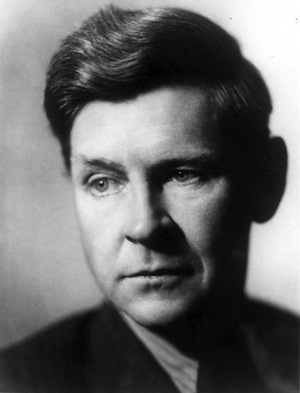
\includegraphics[]{portrait.jpg}\\
width="2.5in" \tabcellsep \noindent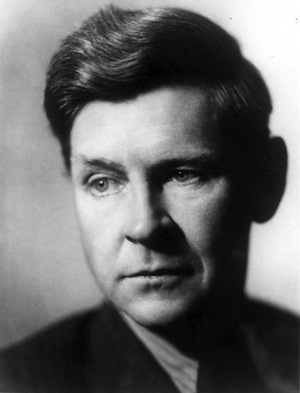
\includegraphics[width=2.5in,]{portrait.jpg}\\
width=".5in" \tabcellsep \noindent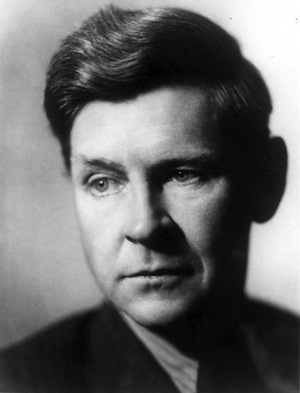
\includegraphics[width=.5in,]{portrait.jpg}\\
scale=".5"\tabcellsep \noindent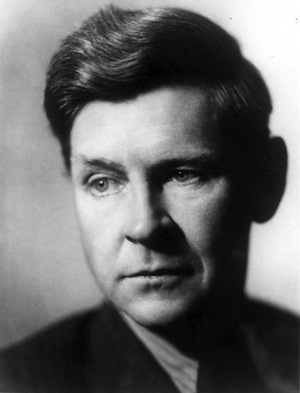
\includegraphics[scale=.5,]{portrait.jpg}\\
width="1in"\tabcellsep \noindent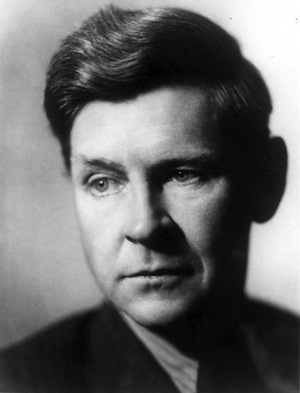
\includegraphics[width=1in,]{portrait.jpg}\\
width="1in" style="border:solid green 	2pt"\tabcellsep \noindent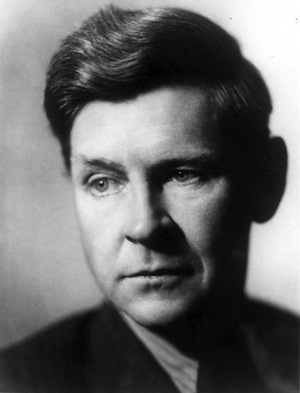
\includegraphics[width=1in,]{portrait.jpg}\\
height="1in"\tabcellsep \noindent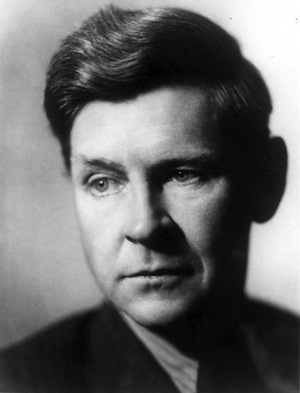
\includegraphics[height=1in,]{portrait.jpg}\\
height="1in" width="2in"\tabcellsep \noindent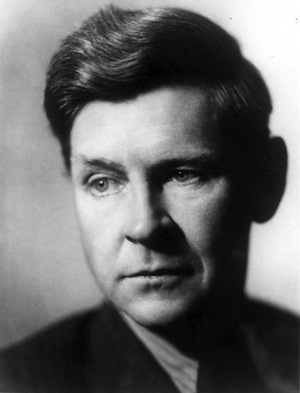
\includegraphics[width=2in,height=1in,]{portrait.jpg}\\
height="2in" width="1in"\tabcellsep \noindent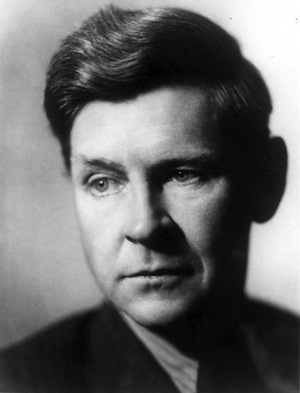
\includegraphics[width=1in,height=2in,]{portrait.jpg}\\
width="10%"\tabcellsep \noindent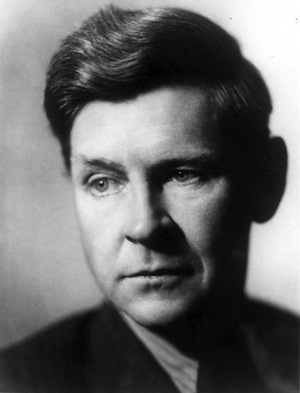
\includegraphics[width=0.1\textwidth,]{portrait.jpg}\\
height="10%" width="10%"\tabcellsep \noindent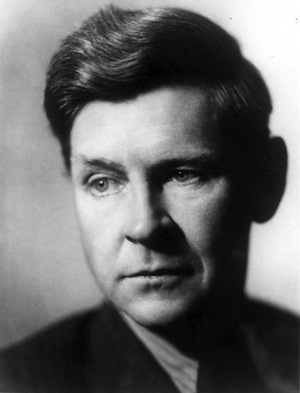
\includegraphics[width=0.1\textwidth,height=0.1\textheight,]{portrait.jpg}\end{longtable} \par
  
\end{document}
